Events at hadron collider are very messy, potentially producing hundreds of particles through many types of physics processes. To illustrate the complexity of such events, a schematic of a proton-proton collision event is shown in Figure~\ref{fig:event}. Two incoming protons collide to create the \emph{hard scatter} shown in red. In this case, two gluons produce a pair of top quarks. The left top decays hadronically and the right decays leptonically. Partons produce radiation as they travel. The hard scatter plus the radiation from the partons is collectively known as the \emph{underlying event}, shown in purple.  Partons are recombined into hadrons (shown as green blobs), a process called \emph{hadronization}. The hadrons can both emit QED radiation (shown in yellow) and then decay further.
\begin{figure}
\centering
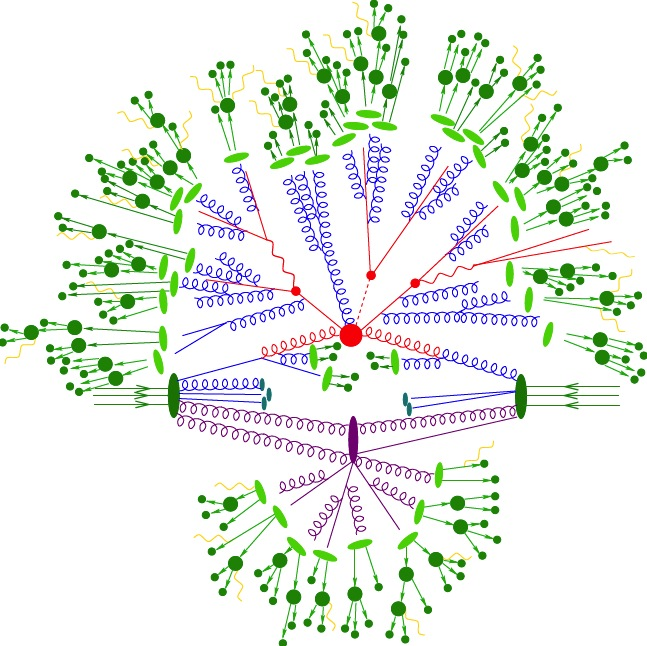
\includegraphics[width=0.8\textwidth]{fig/thry/qcdevent}
\caption{Visualization of a top pair event from the \textsc{Sherpa} event generator. The hard scatter is shown in red, the parton shower in blue, the hadronzation in green, the underlying event in purple, and the QED final state radiation in yellow~\cite{sherpaevent}.}
\label{fig:event}
\end{figure}
The following chapter discusses concepts relevant to analyzing events at hadron colliders. First, terms and concepts in simulating events are introduced. Then, Monte Carlo event generators are discussed. Finally, jet algorithms and concepts are outlined.
% \begin{comment}
\section{Simulation of hadron collisions}

In order to analyze complicated processes at huge machines like the LHC, software that virtually reproduces the physics experiment is necessary. In order to account for stochastic effects, Monte Carlo (MC) methods are used to simulate a large number random events.  In the actual experiment, ATLAS detects collisions produced by the LHC and stores these \emph{events} in a data acquisition system. In the virtual simulation, event generators such as \hw~\cite{Herwig} and \py\cite{pythia6} produce final state particles. These particles are then run through a detector simulation of ATLAS built with \textsc{Geant 4}\cite{bib:g4}. The simulated and actual detector signals can then share the same event reconstruction framework and analysis. This allows a clear understanding of how the input physics is distorted step-by-step as it goes through the detector and reconstruction. 

The distortions resulting from detector imperfections and reconstruction are particularly important to this thesis, so the following chapters will employ specific terms to refer to different aspects of the simulation process. \emph{Generator-level} or \emph{truth} particles refer to those produced by the MC generator before any detector interactions. \emph{Detector-level} or \emph{reconstructed} particles refer to those that have gone through the detector simulation and been reconstructed. 

To go backwards from the (distorted) reconstructed to truth particles, the distortions introduced by the detector must be reversed. This correction process is referred to as \emph{unfolding} and is further discussed in Chapter~\ref{ch:unfolding}. Unfolding is necessary to compare actual data measured with the detector to theoretical predictions produced by generators.
\section{Monte Carlo generators}
In MC event generators, events are produced step-by-step, with random numbers pulled from quantum mechanical probability distributions at various stages\cite{PDG,Sjostrand:2009ad}.  Averaging over a large number of events gives the expected final distribution of events. The goal is to start with a QFT matrix element in a form similar to Equation~\ref{eq:ab} and produce \emph{final state}, stable particles that can be measured with a detector. The method outlines below uses a set of rules at each step to allow the iterative construction of an increasingly complex final state, resulting in hundreds of particles traveling in different directions. Since each particle has $\mathcal{O}(10)$ degrees of freedom (mass, momentum, lifetime, flavor, etc.), each event involves thousands of choices. The result of the simulation must accurately describe the average final state particles as well as fluctuations around the average. 


The steps to generate an event at the LHC can be summarized as follows:
\begin{itemize}
\item Two initial incoming protons are considered as a bag of partons with momentum distributed according to the proton PDFs and specified center of mass energy (in the case of this thesis, 8 \tev).
\item Two partons, one from each proton, are collided to give the \emph{hard process} of interest: $ug \rarrow ug, u\bar{d}\rarrow W^{+}$, etc. If unstable particles such as top quark or $W/Z$ boson are produced, their decay is treated as part of the hard process in order to properly transfer properties such as spin correlations.
\item Just as electromagnetic charges can emit bremsstrahlung, color charges (i.e. partons) can emit QCD radiation. These emissions are collectively called the \emph{parton shower} (PS). Radiation emitted by partons before the collision is called Initial State Radiation (ISR). Radiation emitted by partons after the collision is called Final State Radiation (FSR).  
\item Since the proton is made up of many partons, further parton pairs may collide within a single proton-proton collision, called multiparton interactions (MPI). Each of these further collisions may have ISR or FSR. MPI is different from pileup events, when several protons collide within a single bunch crossing. 
\item After the parton collision, most of the energy remains in the beam remnants, which continue to travel in the original direction and carry color. As the partons from the collision recede, confinement forces come to dominate. These fields cannot be sufficiently described from first principles, so a model must be introduced to describe the evolution of partons into primary hadrons, a process known as \emph{hadronization}. For example, \py\ uses a \emph{string} cluster method, where the confinement field is modeled as a string stretched between each color and its anticolor. Strings are then stretched until it breaks and creates a new pair. This process is repeated until the string energy is sufficiently low-energy and the quarks from adjacent breaks produce primary hadrons. The \emph{cluster} model used by \hw\ groups quark pairs into colorless clusters. These clusters then decay into other colorless clusters or SM hadrons until only SM hadrons remain.
\item Many of these primary hadrons are unstable and decay at different timescales. Some of these decays take place within the detector volume. For ATLAS, particles with $c\tau > 10$ mm are considered \emph{final state} particles. Particles below this threshold are decayed by the event generator. 
\item At this point, the final state particles can be passed on to the detector simulation framework. Experimental information can be used to reconstuct what happened at the core of the process.
\end{itemize}

Produced via the above steps, the cross section for the range of final states produced a hard process of physics interest can be represented schematically as:
\begin{equation}
\sigma_{\text{final state}}=\sigma_{\text{hard process}} \mathcal{P}_{\text{tot, hard process \rarrow final state}}
\label{eq:finalst}
\end{equation}
This equation must be properly integrated over phase-space as well as summed over all possible decay paths that lead to a given final state. The hard process $\sigma_{\text{hard process}}$ can be calculated as in Equation~\ref{eq:ab}. The steps to reach the final state from the hard process are treated probabilistically.


Some of the available event generators go through the complete simulation process while others can only handle some of the steps. General-purpose generators such as \py\, \hw, and \textsc{Sherpa} handle the entire process, from matrix element to PS and hadronization. Other generators such as \textsc{MC@NLO}\cite{mcatnlo,mcatnlo2} and \pow \cite{Powheg,Powheg2,Powheg3,Powheg4} can only generate a fixed order calculation of the hard process and must be interfaced to another generator such as for \py\ or \hw for the PS. 

Merging the hard process calculation with a PS program can be tricky. Both may produce wide angle radiation, so care must be taken not to double count partons. For NLO+PS, double counting can happen because PS programs attempt to emulate effects of a true NLO calculate. Two different methods are used in \textsc{MC@NLO}\ and \pow\ to avoid double-dounting. \textsc{MC@NLO} uses an analytic computation to identify what parts of the NLO calculation is already present in the PS and then subtracting this portion from the shower before combining. This method requires a new calculation for each PS program since each PS uses different NLO approximations. For \pow, the probability of each iterative spread of the shower is modified for the first emission such that exact NLO accurancy is reached. Then, any PS program can be used to shower the rest of the event with a \pt\ veto to ensure that the PS program doesn't produce any emissions harder than those from the NLO.

Finally, ``afterburner'' programs can be used to more accurately redecay special particles, such as \textsc{Tauola} for taus\cite{Jadach:1993hs} or \textsc{EvtGen} for heavy flavor hadrons\cite{Lange:2001uf}. Though not relevant for this thesis, studies of the effect of \textsc{EvtGen} on the modelling of heavy flavor decays and hadronization is presented in Appendix~\ref{app:evtgen}.

Predictions from generators can be \emph{tuned} by tweaking parameters to match experimental data\cite{Buckley:2009vk}. Each generator has $\mathcal{O}(20-30)$ relatively free parameters, mostly in the non-pertubative hadronization process but also in the pertubative hard interaction. All of these parameters have a physical motivation, but are usually only rough scale approximations. Some parameters like $\alpha_S$ can be measured experimentally but still must be adjusted since generators use them in a fixed-order scheme, unlike nature. These parameters can be grouped into sets such as flavor, fragmentation, hard process, etc. Most of the hard process parameters are tunes to Tevatron and LHC data, while most of the hadronization parameters come from LEP. The measurement of this thesis is important for future tuning of PS parameters since additional jets are sensitive to ISR/FSR.

\section{Jets}
Partons cannot be directly observed at the LHC since QCD confinement prevents partons from existing as free particles. Instead, narrow cones of hadrons and other particles from the hadronization of a parton are experimentally studied to determine the properties of the original parton. These cones are identified as experimentally observable objects called jets. Ideally, each jet would match with a parton shower initiated by a single hard parton. However, a jet may contain parts of showers from multiple partons and ISR/FSR. 

Since a jet is not a fundamental physics object, a suitable definition must be adopted to analyze them. A \emph{jet algorithm} used to build jets from final state particles in the generator record, charged particle tracks or energy deposits in the calorimeter. A good jet algorithm must be~\cite{Atkin:2015msa}
\begin{itemize}
\item Simple to implement for experimental analysis;
\item Simple to implement for theoretical calculation;
\item Defined at any order of pertubation theory;
\item Yield finite cross sections at any order of pertubatiion theory;
\item Yield cross sections relatively insensitive to hadronization model
\item Infared and collinear (IRC) safe, e.g. jets should be stable under modification of final state particles via soft emissions or collinear splitting to avoid infinite results in calculations due to infrared divergences
\end{itemize}

Modern jet algorithm specifies the way the 4-vectors of the input constituents are combined with a distance metric. The standard algorithm used by both ATLAS and CMS is the \akt jet algorithm\cite{antikt1,antikt2}, which fulfills the above criteria exceedingly well. The \kt\ algorithm is a closely related algorithm used in special cases with irregular jets. 

The \akt\ algorithm begins by defining the distances between two constituents $i$ and $j$ and between constituents $i$ and the beam as:
\begin{flalign}
d_{ij} &= \mbox{min}(p^{2k}_{T,i}, p^{2k}_{T,j})\left(\frac{\Delta R_{ij}}{R_0}\right)^2\\
d_{iB} &= p^{2k}_{T,i}
\end{flalign}
where $p_T$ is the transverse momentum of the constituent, $\Delta R_{ij}\equiv \sqrt{(\eta_i - \eta_j)^2 + (\phi_i - \phi_j)^2}$ and $R_0$ is a chosen parameter that approximately determines the jet in the $\eta-\phi$ plane. The \akt\ and \kt\ algorithm differ only in the choice for the exponent $k$. For \kt, $k=+1$ and for \akt\ $k=-1$. 

With a chosen distance metric and set of input constituents, the algorithm iteratively proceeds as follows:
\begin{itemize}
\item find the smallest $d_{ij}$ and $d_{iB}$
\item if $d_{ij} < d_{iB}$, replace $i$ and $j$ by a new constituent formed by the 4-vector sum of $i$ and $j$ 
\item if $d_{ij} > d_{iB}$, declare $i$ a jet and remove from the list of constituents
\end{itemize}

Figure~\ref{fig:ktalg} shows the results of clustering the same set of constituents with each of these algorithms. The difference between the two can be roughly explained by observing that \kt\ clusters the lower \pt\ constituents first, while \akt\ clusters the higher \pt\ constituents first. Since \akt\ takes the highest \pt\ constituents first, the jet axis stabilizes after the first few combination and results in circular jets. Circular jets have better defined acceptance and are easier to calibrate. This feature of the \akt\ algorithm motivates its adoption as the ATLAS default and its use in this thesis.

\begin{figure}[h]
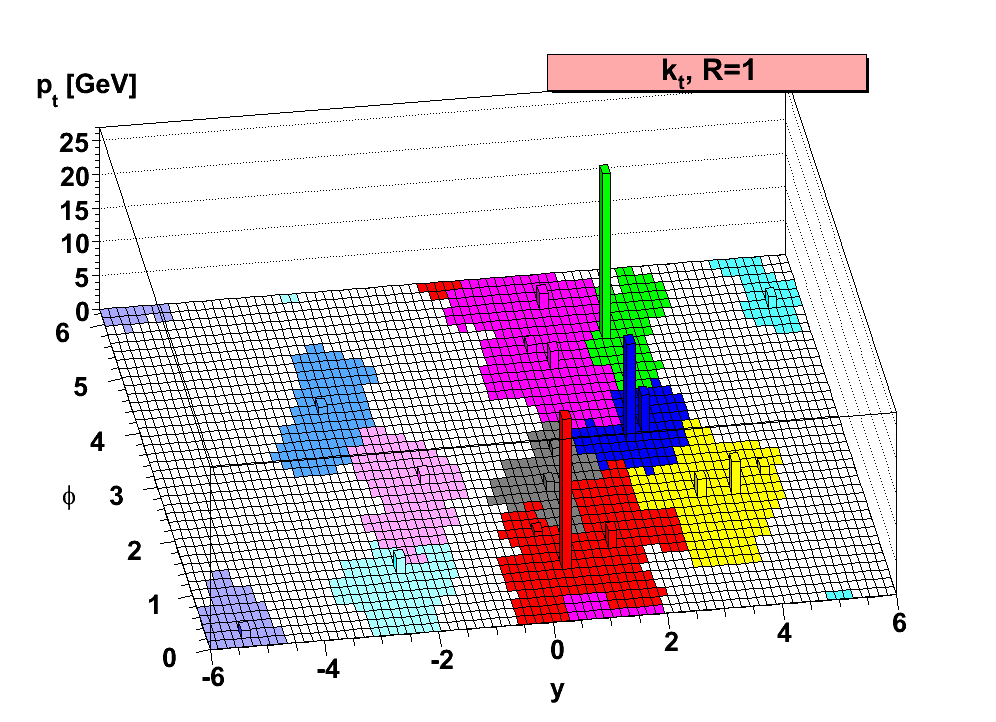
\includegraphics[width=0.5\textwidth]{fig/thry/kt.png}
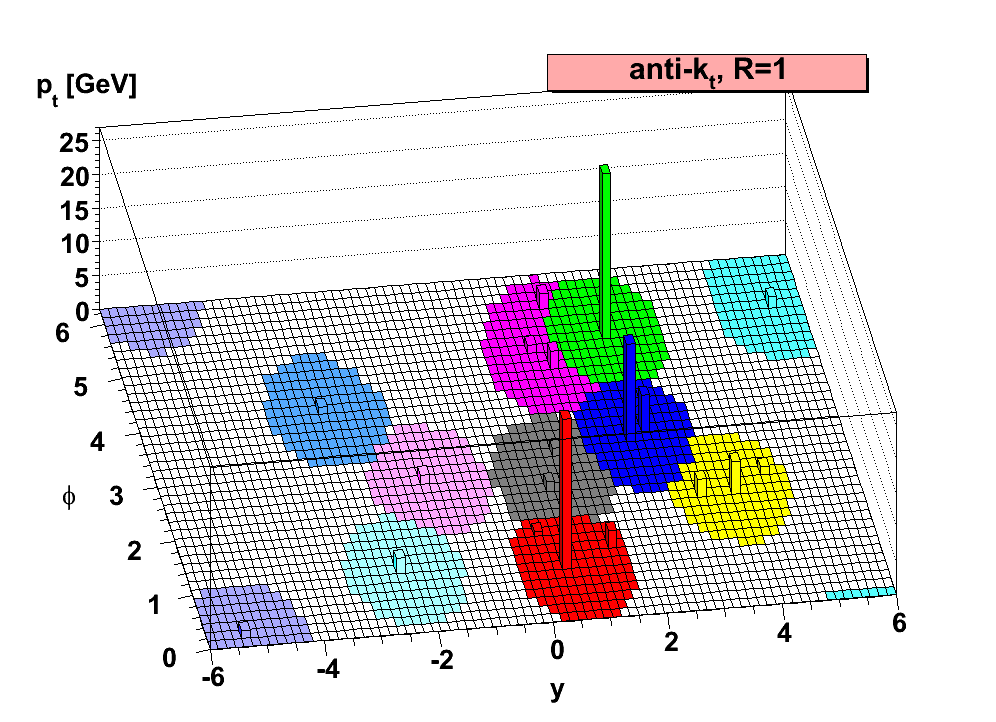
\includegraphics[width=0.5\textwidth]{fig/thry/antikt.png}
\caption{The input constituents clustered both the \kt (left) and the \akt (right) algorithms~\cite{antikt1}.}
\label{fig:ktalg}
\end{figure}

